% Created by tikzDevice version 0.12.6 on 2025-02-15 09:16:45
% !TEX encoding = UTF-8 Unicode
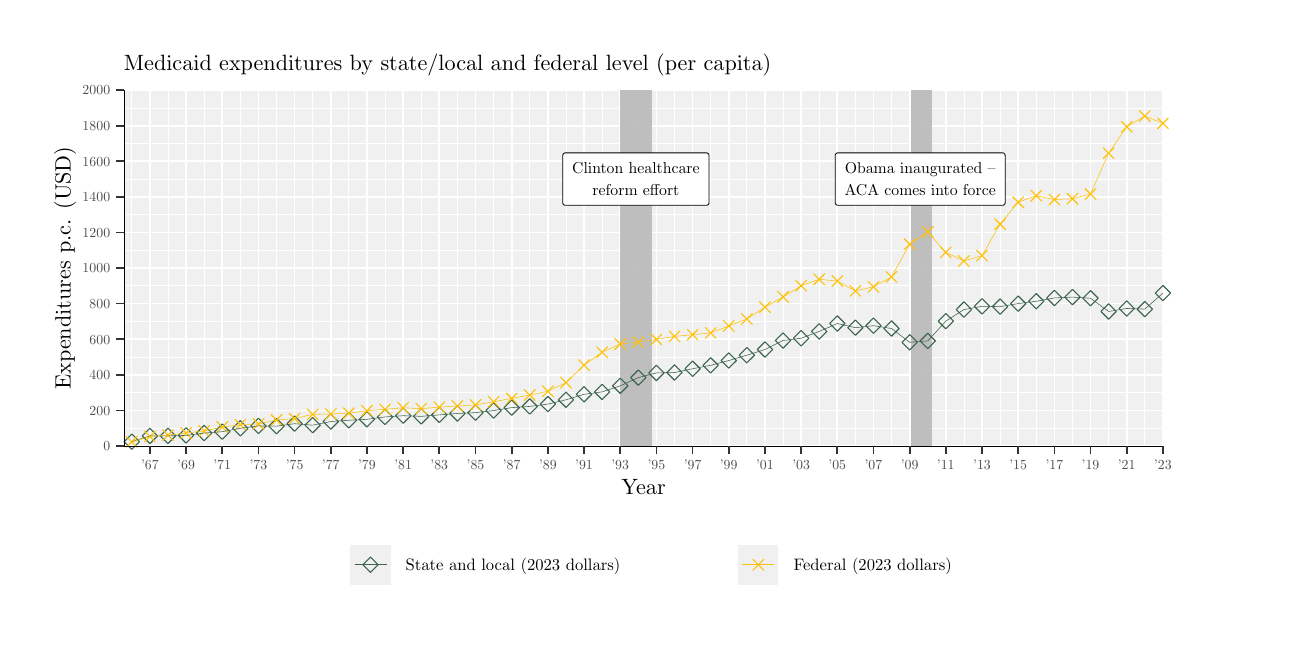
\begin{tikzpicture}[x=1pt,y=1pt]
\definecolor{fillColor}{RGB}{255,255,255}
\path[use as bounding box,fill=fillColor,fill opacity=0.00] (0,0) rectangle (455.30,216.81);
\begin{scope}
\path[clip] (  0.00,  0.00) rectangle (455.30,216.81);
\definecolor{drawColor}{RGB}{255,255,255}
\definecolor{fillColor}{RGB}{255,255,255}

\path[draw=drawColor,line width= 0.6pt,line join=round,line cap=round,fill=fillColor] (  0.00,  0.00) rectangle (455.30,216.81);
\end{scope}
\begin{scope}
\path[clip] (  0.00,  0.00) rectangle (455.30,216.81);
\definecolor{fillColor}{gray}{0.94}

\path[fill=fillColor] ( 34.76, 65.63) rectangle (410.30,194.25);
\definecolor{drawColor}{RGB}{255,255,255}

\path[draw=drawColor,line width= 0.3pt,line join=round] ( 34.76, 72.07) --
	(410.30, 72.07);

\path[draw=drawColor,line width= 0.3pt,line join=round] ( 34.76, 84.93) --
	(410.30, 84.93);

\path[draw=drawColor,line width= 0.3pt,line join=round] ( 34.76, 97.79) --
	(410.30, 97.79);

\path[draw=drawColor,line width= 0.3pt,line join=round] ( 34.76,110.65) --
	(410.30,110.65);

\path[draw=drawColor,line width= 0.3pt,line join=round] ( 34.76,123.51) --
	(410.30,123.51);

\path[draw=drawColor,line width= 0.3pt,line join=round] ( 34.76,136.37) --
	(410.30,136.37);

\path[draw=drawColor,line width= 0.3pt,line join=round] ( 34.76,149.23) --
	(410.30,149.23);

\path[draw=drawColor,line width= 0.3pt,line join=round] ( 34.76,162.09) --
	(410.30,162.09);

\path[draw=drawColor,line width= 0.3pt,line join=round] ( 34.76,174.95) --
	(410.30,174.95);

\path[draw=drawColor,line width= 0.3pt,line join=round] ( 34.76,187.81) --
	(410.30,187.81);

\path[draw=drawColor,line width= 0.3pt,line join=round] ( 37.63, 65.63) --
	( 37.63,194.25);

\path[draw=drawColor,line width= 0.3pt,line join=round] ( 50.70, 65.63) --
	( 50.70,194.25);

\path[draw=drawColor,line width= 0.3pt,line join=round] ( 63.77, 65.63) --
	( 63.77,194.25);

\path[draw=drawColor,line width= 0.3pt,line join=round] ( 76.85, 65.63) --
	( 76.85,194.25);

\path[draw=drawColor,line width= 0.3pt,line join=round] ( 89.92, 65.63) --
	( 89.92,194.25);

\path[draw=drawColor,line width= 0.3pt,line join=round] (102.99, 65.63) --
	(102.99,194.25);

\path[draw=drawColor,line width= 0.3pt,line join=round] (116.07, 65.63) --
	(116.07,194.25);

\path[draw=drawColor,line width= 0.3pt,line join=round] (129.14, 65.63) --
	(129.14,194.25);

\path[draw=drawColor,line width= 0.3pt,line join=round] (142.21, 65.63) --
	(142.21,194.25);

\path[draw=drawColor,line width= 0.3pt,line join=round] (155.29, 65.63) --
	(155.29,194.25);

\path[draw=drawColor,line width= 0.3pt,line join=round] (168.36, 65.63) --
	(168.36,194.25);

\path[draw=drawColor,line width= 0.3pt,line join=round] (181.43, 65.63) --
	(181.43,194.25);

\path[draw=drawColor,line width= 0.3pt,line join=round] (194.51, 65.63) --
	(194.51,194.25);

\path[draw=drawColor,line width= 0.3pt,line join=round] (207.58, 65.63) --
	(207.58,194.25);

\path[draw=drawColor,line width= 0.3pt,line join=round] (220.65, 65.63) --
	(220.65,194.25);

\path[draw=drawColor,line width= 0.3pt,line join=round] (233.73, 65.63) --
	(233.73,194.25);

\path[draw=drawColor,line width= 0.3pt,line join=round] (246.80, 65.63) --
	(246.80,194.25);

\path[draw=drawColor,line width= 0.3pt,line join=round] (259.87, 65.63) --
	(259.87,194.25);

\path[draw=drawColor,line width= 0.3pt,line join=round] (272.95, 65.63) --
	(272.95,194.25);

\path[draw=drawColor,line width= 0.3pt,line join=round] (286.02, 65.63) --
	(286.02,194.25);

\path[draw=drawColor,line width= 0.3pt,line join=round] (299.09, 65.63) --
	(299.09,194.25);

\path[draw=drawColor,line width= 0.3pt,line join=round] (312.17, 65.63) --
	(312.17,194.25);

\path[draw=drawColor,line width= 0.3pt,line join=round] (325.24, 65.63) --
	(325.24,194.25);

\path[draw=drawColor,line width= 0.3pt,line join=round] (338.31, 65.63) --
	(338.31,194.25);

\path[draw=drawColor,line width= 0.3pt,line join=round] (351.39, 65.63) --
	(351.39,194.25);

\path[draw=drawColor,line width= 0.3pt,line join=round] (364.46, 65.63) --
	(364.46,194.25);

\path[draw=drawColor,line width= 0.3pt,line join=round] (377.53, 65.63) --
	(377.53,194.25);

\path[draw=drawColor,line width= 0.3pt,line join=round] (390.61, 65.63) --
	(390.61,194.25);

\path[draw=drawColor,line width= 0.3pt,line join=round] (403.68, 65.63) --
	(403.68,194.25);

\path[draw=drawColor,line width= 0.6pt,line join=round] ( 34.76, 65.63) --
	(410.30, 65.63);

\path[draw=drawColor,line width= 0.6pt,line join=round] ( 34.76, 78.50) --
	(410.30, 78.50);

\path[draw=drawColor,line width= 0.6pt,line join=round] ( 34.76, 91.36) --
	(410.30, 91.36);

\path[draw=drawColor,line width= 0.6pt,line join=round] ( 34.76,104.22) --
	(410.30,104.22);

\path[draw=drawColor,line width= 0.6pt,line join=round] ( 34.76,117.08) --
	(410.30,117.08);

\path[draw=drawColor,line width= 0.6pt,line join=round] ( 34.76,129.94) --
	(410.30,129.94);

\path[draw=drawColor,line width= 0.6pt,line join=round] ( 34.76,142.80) --
	(410.30,142.80);

\path[draw=drawColor,line width= 0.6pt,line join=round] ( 34.76,155.66) --
	(410.30,155.66);

\path[draw=drawColor,line width= 0.6pt,line join=round] ( 34.76,168.52) --
	(410.30,168.52);

\path[draw=drawColor,line width= 0.6pt,line join=round] ( 34.76,181.38) --
	(410.30,181.38);

\path[draw=drawColor,line width= 0.6pt,line join=round] ( 34.76,194.25) --
	(410.30,194.25);

\path[draw=drawColor,line width= 0.6pt,line join=round] ( 44.16, 65.63) --
	( 44.16,194.25);

\path[draw=drawColor,line width= 0.6pt,line join=round] ( 57.24, 65.63) --
	( 57.24,194.25);

\path[draw=drawColor,line width= 0.6pt,line join=round] ( 70.30, 65.63) --
	( 70.30,194.25);

\path[draw=drawColor,line width= 0.6pt,line join=round] ( 83.39, 65.63) --
	( 83.39,194.25);

\path[draw=drawColor,line width= 0.6pt,line join=round] ( 96.45, 65.63) --
	( 96.45,194.25);

\path[draw=drawColor,line width= 0.6pt,line join=round] (109.53, 65.63) --
	(109.53,194.25);

\path[draw=drawColor,line width= 0.6pt,line join=round] (122.60, 65.63) --
	(122.60,194.25);

\path[draw=drawColor,line width= 0.6pt,line join=round] (135.68, 65.63) --
	(135.68,194.25);

\path[draw=drawColor,line width= 0.6pt,line join=round] (148.74, 65.63) --
	(148.74,194.25);

\path[draw=drawColor,line width= 0.6pt,line join=round] (161.83, 65.63) --
	(161.83,194.25);

\path[draw=drawColor,line width= 0.6pt,line join=round] (174.89, 65.63) --
	(174.89,194.25);

\path[draw=drawColor,line width= 0.6pt,line join=round] (187.97, 65.63) --
	(187.97,194.25);

\path[draw=drawColor,line width= 0.6pt,line join=round] (201.04, 65.63) --
	(201.04,194.25);

\path[draw=drawColor,line width= 0.6pt,line join=round] (214.12, 65.63) --
	(214.12,194.25);

\path[draw=drawColor,line width= 0.6pt,line join=round] (227.18, 65.63) --
	(227.18,194.25);

\path[draw=drawColor,line width= 0.6pt,line join=round] (240.27, 65.63) --
	(240.27,194.25);

\path[draw=drawColor,line width= 0.6pt,line join=round] (253.33, 65.63) --
	(253.33,194.25);

\path[draw=drawColor,line width= 0.6pt,line join=round] (266.41, 65.63) --
	(266.41,194.25);

\path[draw=drawColor,line width= 0.6pt,line join=round] (279.48, 65.63) --
	(279.48,194.25);

\path[draw=drawColor,line width= 0.6pt,line join=round] (292.56, 65.63) --
	(292.56,194.25);

\path[draw=drawColor,line width= 0.6pt,line join=round] (305.62, 65.63) --
	(305.62,194.25);

\path[draw=drawColor,line width= 0.6pt,line join=round] (318.71, 65.63) --
	(318.71,194.25);

\path[draw=drawColor,line width= 0.6pt,line join=round] (331.77, 65.63) --
	(331.77,194.25);

\path[draw=drawColor,line width= 0.6pt,line join=round] (344.85, 65.63) --
	(344.85,194.25);

\path[draw=drawColor,line width= 0.6pt,line join=round] (357.92, 65.63) --
	(357.92,194.25);

\path[draw=drawColor,line width= 0.6pt,line join=round] (371.00, 65.63) --
	(371.00,194.25);

\path[draw=drawColor,line width= 0.6pt,line join=round] (384.06, 65.63) --
	(384.06,194.25);

\path[draw=drawColor,line width= 0.6pt,line join=round] (397.15, 65.63) --
	(397.15,194.25);

\path[draw=drawColor,line width= 0.6pt,line join=round] (410.21, 65.63) --
	(410.21,194.25);
\definecolor{drawColor}{RGB}{190,190,190}

\path[draw=drawColor,line width= 0.6pt,line join=round] ( -1.60, 65.63) -- ( -1.60,194.25);
\definecolor{fillColor}{RGB}{190,190,190}

\path[fill=fillColor,fill opacity=0.01] (214.12, 65.63) rectangle (225.45,194.25);

\path[fill=fillColor,fill opacity=0.01] (214.12, 65.63) rectangle (225.45,194.25);

\path[fill=fillColor,fill opacity=0.01] (214.12, 65.63) rectangle (225.45,194.25);

\path[fill=fillColor,fill opacity=0.01] (214.12, 65.63) rectangle (225.45,194.25);

\path[fill=fillColor,fill opacity=0.01] (214.12, 65.63) rectangle (225.45,194.25);

\path[fill=fillColor,fill opacity=0.01] (214.12, 65.63) rectangle (225.45,194.25);

\path[fill=fillColor,fill opacity=0.01] (214.12, 65.63) rectangle (225.45,194.25);

\path[fill=fillColor,fill opacity=0.01] (214.12, 65.63) rectangle (225.45,194.25);

\path[fill=fillColor,fill opacity=0.01] (214.12, 65.63) rectangle (225.45,194.25);

\path[fill=fillColor,fill opacity=0.01] (214.12, 65.63) rectangle (225.45,194.25);

\path[fill=fillColor,fill opacity=0.01] (214.12, 65.63) rectangle (225.45,194.25);

\path[fill=fillColor,fill opacity=0.01] (214.12, 65.63) rectangle (225.45,194.25);

\path[fill=fillColor,fill opacity=0.01] (214.12, 65.63) rectangle (225.45,194.25);

\path[fill=fillColor,fill opacity=0.01] (214.12, 65.63) rectangle (225.45,194.25);

\path[fill=fillColor,fill opacity=0.01] (214.12, 65.63) rectangle (225.45,194.25);

\path[fill=fillColor,fill opacity=0.01] (214.12, 65.63) rectangle (225.45,194.25);

\path[fill=fillColor,fill opacity=0.01] (214.12, 65.63) rectangle (225.45,194.25);

\path[fill=fillColor,fill opacity=0.01] (214.12, 65.63) rectangle (225.45,194.25);

\path[fill=fillColor,fill opacity=0.01] (214.12, 65.63) rectangle (225.45,194.25);

\path[fill=fillColor,fill opacity=0.01] (214.12, 65.63) rectangle (225.45,194.25);

\path[fill=fillColor,fill opacity=0.01] (214.12, 65.63) rectangle (225.45,194.25);

\path[fill=fillColor,fill opacity=0.01] (214.12, 65.63) rectangle (225.45,194.25);

\path[fill=fillColor,fill opacity=0.01] (214.12, 65.63) rectangle (225.45,194.25);

\path[fill=fillColor,fill opacity=0.01] (214.12, 65.63) rectangle (225.45,194.25);

\path[fill=fillColor,fill opacity=0.01] (214.12, 65.63) rectangle (225.45,194.25);

\path[fill=fillColor,fill opacity=0.01] (214.12, 65.63) rectangle (225.45,194.25);

\path[fill=fillColor,fill opacity=0.01] (214.12, 65.63) rectangle (225.45,194.25);

\path[fill=fillColor,fill opacity=0.01] (214.12, 65.63) rectangle (225.45,194.25);

\path[fill=fillColor,fill opacity=0.01] (214.12, 65.63) rectangle (225.45,194.25);

\path[fill=fillColor,fill opacity=0.01] (214.12, 65.63) rectangle (225.45,194.25);

\path[fill=fillColor,fill opacity=0.01] (214.12, 65.63) rectangle (225.45,194.25);

\path[fill=fillColor,fill opacity=0.01] (214.12, 65.63) rectangle (225.45,194.25);

\path[fill=fillColor,fill opacity=0.01] (214.12, 65.63) rectangle (225.45,194.25);

\path[fill=fillColor,fill opacity=0.01] (214.12, 65.63) rectangle (225.45,194.25);

\path[fill=fillColor,fill opacity=0.01] (214.12, 65.63) rectangle (225.45,194.25);

\path[fill=fillColor,fill opacity=0.01] (214.12, 65.63) rectangle (225.45,194.25);

\path[fill=fillColor,fill opacity=0.01] (214.12, 65.63) rectangle (225.45,194.25);

\path[fill=fillColor,fill opacity=0.01] (214.12, 65.63) rectangle (225.45,194.25);

\path[fill=fillColor,fill opacity=0.01] (214.12, 65.63) rectangle (225.45,194.25);

\path[fill=fillColor,fill opacity=0.01] (214.12, 65.63) rectangle (225.45,194.25);

\path[fill=fillColor,fill opacity=0.01] (214.12, 65.63) rectangle (225.45,194.25);

\path[fill=fillColor,fill opacity=0.01] (214.12, 65.63) rectangle (225.45,194.25);

\path[fill=fillColor,fill opacity=0.01] (214.12, 65.63) rectangle (225.45,194.25);

\path[fill=fillColor,fill opacity=0.01] (214.12, 65.63) rectangle (225.45,194.25);

\path[fill=fillColor,fill opacity=0.01] (214.12, 65.63) rectangle (225.45,194.25);

\path[fill=fillColor,fill opacity=0.01] (214.12, 65.63) rectangle (225.45,194.25);

\path[fill=fillColor,fill opacity=0.01] (214.12, 65.63) rectangle (225.45,194.25);

\path[fill=fillColor,fill opacity=0.01] (214.12, 65.63) rectangle (225.45,194.25);

\path[fill=fillColor,fill opacity=0.01] (214.12, 65.63) rectangle (225.45,194.25);

\path[fill=fillColor,fill opacity=0.01] (214.12, 65.63) rectangle (225.45,194.25);

\path[fill=fillColor,fill opacity=0.01] (214.12, 65.63) rectangle (225.45,194.25);

\path[fill=fillColor,fill opacity=0.01] (214.12, 65.63) rectangle (225.45,194.25);

\path[fill=fillColor,fill opacity=0.01] (214.12, 65.63) rectangle (225.45,194.25);

\path[fill=fillColor,fill opacity=0.01] (214.12, 65.63) rectangle (225.45,194.25);

\path[fill=fillColor,fill opacity=0.01] (214.12, 65.63) rectangle (225.45,194.25);

\path[fill=fillColor,fill opacity=0.01] (214.12, 65.63) rectangle (225.45,194.25);

\path[fill=fillColor,fill opacity=0.01] (214.12, 65.63) rectangle (225.45,194.25);

\path[fill=fillColor,fill opacity=0.01] (214.12, 65.63) rectangle (225.45,194.25);

\path[fill=fillColor,fill opacity=0.01] (214.12, 65.63) rectangle (225.45,194.25);

\path[fill=fillColor,fill opacity=0.01] (214.12, 65.63) rectangle (225.45,194.25);

\path[fill=fillColor,fill opacity=0.01] (214.12, 65.63) rectangle (225.45,194.25);

\path[fill=fillColor,fill opacity=0.01] (214.12, 65.63) rectangle (225.45,194.25);

\path[fill=fillColor,fill opacity=0.01] (214.12, 65.63) rectangle (225.45,194.25);

\path[fill=fillColor,fill opacity=0.01] (214.12, 65.63) rectangle (225.45,194.25);

\path[fill=fillColor,fill opacity=0.01] (319.05, 65.63) rectangle (326.69,194.25);

\path[fill=fillColor,fill opacity=0.01] (319.05, 65.63) rectangle (326.69,194.25);

\path[fill=fillColor,fill opacity=0.01] (319.05, 65.63) rectangle (326.69,194.25);

\path[fill=fillColor,fill opacity=0.01] (319.05, 65.63) rectangle (326.69,194.25);

\path[fill=fillColor,fill opacity=0.01] (319.05, 65.63) rectangle (326.69,194.25);

\path[fill=fillColor,fill opacity=0.01] (319.05, 65.63) rectangle (326.69,194.25);

\path[fill=fillColor,fill opacity=0.01] (319.05, 65.63) rectangle (326.69,194.25);

\path[fill=fillColor,fill opacity=0.01] (319.05, 65.63) rectangle (326.69,194.25);

\path[fill=fillColor,fill opacity=0.01] (319.05, 65.63) rectangle (326.69,194.25);

\path[fill=fillColor,fill opacity=0.01] (319.05, 65.63) rectangle (326.69,194.25);

\path[fill=fillColor,fill opacity=0.01] (319.05, 65.63) rectangle (326.69,194.25);

\path[fill=fillColor,fill opacity=0.01] (319.05, 65.63) rectangle (326.69,194.25);

\path[fill=fillColor,fill opacity=0.01] (319.05, 65.63) rectangle (326.69,194.25);

\path[fill=fillColor,fill opacity=0.01] (319.05, 65.63) rectangle (326.69,194.25);

\path[fill=fillColor,fill opacity=0.01] (319.05, 65.63) rectangle (326.69,194.25);

\path[fill=fillColor,fill opacity=0.01] (319.05, 65.63) rectangle (326.69,194.25);

\path[fill=fillColor,fill opacity=0.01] (319.05, 65.63) rectangle (326.69,194.25);

\path[fill=fillColor,fill opacity=0.01] (319.05, 65.63) rectangle (326.69,194.25);

\path[fill=fillColor,fill opacity=0.01] (319.05, 65.63) rectangle (326.69,194.25);

\path[fill=fillColor,fill opacity=0.01] (319.05, 65.63) rectangle (326.69,194.25);

\path[fill=fillColor,fill opacity=0.01] (319.05, 65.63) rectangle (326.69,194.25);

\path[fill=fillColor,fill opacity=0.01] (319.05, 65.63) rectangle (326.69,194.25);

\path[fill=fillColor,fill opacity=0.01] (319.05, 65.63) rectangle (326.69,194.25);

\path[fill=fillColor,fill opacity=0.01] (319.05, 65.63) rectangle (326.69,194.25);

\path[fill=fillColor,fill opacity=0.01] (319.05, 65.63) rectangle (326.69,194.25);

\path[fill=fillColor,fill opacity=0.01] (319.05, 65.63) rectangle (326.69,194.25);

\path[fill=fillColor,fill opacity=0.01] (319.05, 65.63) rectangle (326.69,194.25);

\path[fill=fillColor,fill opacity=0.01] (319.05, 65.63) rectangle (326.69,194.25);

\path[fill=fillColor,fill opacity=0.01] (319.05, 65.63) rectangle (326.69,194.25);

\path[fill=fillColor,fill opacity=0.01] (319.05, 65.63) rectangle (326.69,194.25);

\path[fill=fillColor,fill opacity=0.01] (319.05, 65.63) rectangle (326.69,194.25);

\path[fill=fillColor,fill opacity=0.01] (319.05, 65.63) rectangle (326.69,194.25);

\path[fill=fillColor,fill opacity=0.01] (319.05, 65.63) rectangle (326.69,194.25);

\path[fill=fillColor,fill opacity=0.01] (319.05, 65.63) rectangle (326.69,194.25);

\path[fill=fillColor,fill opacity=0.01] (319.05, 65.63) rectangle (326.69,194.25);

\path[fill=fillColor,fill opacity=0.01] (319.05, 65.63) rectangle (326.69,194.25);

\path[fill=fillColor,fill opacity=0.01] (319.05, 65.63) rectangle (326.69,194.25);

\path[fill=fillColor,fill opacity=0.01] (319.05, 65.63) rectangle (326.69,194.25);

\path[fill=fillColor,fill opacity=0.01] (319.05, 65.63) rectangle (326.69,194.25);

\path[fill=fillColor,fill opacity=0.01] (319.05, 65.63) rectangle (326.69,194.25);

\path[fill=fillColor,fill opacity=0.01] (319.05, 65.63) rectangle (326.69,194.25);

\path[fill=fillColor,fill opacity=0.01] (319.05, 65.63) rectangle (326.69,194.25);

\path[fill=fillColor,fill opacity=0.01] (319.05, 65.63) rectangle (326.69,194.25);

\path[fill=fillColor,fill opacity=0.01] (319.05, 65.63) rectangle (326.69,194.25);

\path[fill=fillColor,fill opacity=0.01] (319.05, 65.63) rectangle (326.69,194.25);

\path[fill=fillColor,fill opacity=0.01] (319.05, 65.63) rectangle (326.69,194.25);

\path[fill=fillColor,fill opacity=0.01] (319.05, 65.63) rectangle (326.69,194.25);

\path[fill=fillColor,fill opacity=0.01] (319.05, 65.63) rectangle (326.69,194.25);

\path[fill=fillColor,fill opacity=0.01] (319.05, 65.63) rectangle (326.69,194.25);

\path[fill=fillColor,fill opacity=0.01] (319.05, 65.63) rectangle (326.69,194.25);

\path[fill=fillColor,fill opacity=0.01] (319.05, 65.63) rectangle (326.69,194.25);

\path[fill=fillColor,fill opacity=0.01] (319.05, 65.63) rectangle (326.69,194.25);

\path[fill=fillColor,fill opacity=0.01] (319.05, 65.63) rectangle (326.69,194.25);

\path[fill=fillColor,fill opacity=0.01] (319.05, 65.63) rectangle (326.69,194.25);

\path[fill=fillColor,fill opacity=0.01] (319.05, 65.63) rectangle (326.69,194.25);

\path[fill=fillColor,fill opacity=0.01] (319.05, 65.63) rectangle (326.69,194.25);

\path[fill=fillColor,fill opacity=0.01] (319.05, 65.63) rectangle (326.69,194.25);

\path[fill=fillColor,fill opacity=0.01] (319.05, 65.63) rectangle (326.69,194.25);

\path[fill=fillColor,fill opacity=0.01] (319.05, 65.63) rectangle (326.69,194.25);

\path[fill=fillColor,fill opacity=0.01] (319.05, 65.63) rectangle (326.69,194.25);

\path[fill=fillColor,fill opacity=0.01] (319.05, 65.63) rectangle (326.69,194.25);

\path[fill=fillColor,fill opacity=0.01] (319.05, 65.63) rectangle (326.69,194.25);

\path[fill=fillColor,fill opacity=0.01] (319.05, 65.63) rectangle (326.69,194.25);

\path[fill=fillColor,fill opacity=0.01] (319.05, 65.63) rectangle (326.69,194.25);
\definecolor{drawColor}{RGB}{0,0,0}
\definecolor{fillColor}{RGB}{255,255,255}

\path[draw=drawColor,line width= 0.3pt,line join=round,line cap=round,fill=fillColor] (194.37,152.61) --
	(245.18,152.61) --
	(245.14,152.61) --
	(245.30,152.62) --
	(245.46,152.65) --
	(245.62,152.71) --
	(245.76,152.79) --
	(245.89,152.89) --
	(246.00,153.02) --
	(246.09,153.16) --
	(246.15,153.31) --
	(246.19,153.47) --
	(246.21,153.64) --
	(246.21,153.64) --
	(246.21,170.55) --
	(246.21,170.55) --
	(246.19,170.71) --
	(246.15,170.87) --
	(246.09,171.03) --
	(246.00,171.17) --
	(245.89,171.29) --
	(245.76,171.39) --
	(245.62,171.48) --
	(245.46,171.54) --
	(245.30,171.57) --
	(245.18,171.58) --
	(194.37,171.58) --
	(194.50,171.57) --
	(194.33,171.58) --
	(194.17,171.56) --
	(194.01,171.51) --
	(193.86,171.44) --
	(193.72,171.34) --
	(193.60,171.23) --
	(193.50,171.10) --
	(193.43,170.95) --
	(193.37,170.79) --
	(193.35,170.63) --
	(193.34,170.55) --
	(193.34,153.64) --
	(193.35,153.72) --
	(193.35,153.55) --
	(193.37,153.39) --
	(193.43,153.23) --
	(193.50,153.09) --
	(193.60,152.95) --
	(193.72,152.84) --
	(193.86,152.75) --
	(194.01,152.68) --
	(194.17,152.63) --
	(194.33,152.61) --
	cycle;
\end{scope}
\begin{scope}
\path[clip] (  0.00,  0.00) rectangle (455.30,216.81);
\definecolor{drawColor}{RGB}{0,0,0}

\node[text=drawColor,anchor=base,inner sep=0pt, outer sep=0pt, scale=  0.57] at (219.78,164.23) {Clinton healthcare };

\node[text=drawColor,anchor=base,inner sep=0pt, outer sep=0pt, scale=  0.57] at (219.78,156.04) { reform effort};
\end{scope}
\begin{scope}
\path[clip] (  0.00,  0.00) rectangle (455.30,216.81);
\definecolor{drawColor}{RGB}{0,0,0}
\definecolor{fillColor}{RGB}{255,255,255}

\path[draw=drawColor,line width= 0.3pt,line join=round,line cap=round,fill=fillColor] (292.82,152.61) --
	(352.19,152.61) --
	(352.15,152.61) --
	(352.31,152.62) --
	(352.47,152.65) --
	(352.63,152.71) --
	(352.77,152.79) --
	(352.90,152.89) --
	(353.01,153.02) --
	(353.10,153.16) --
	(353.16,153.31) --
	(353.20,153.47) --
	(353.22,153.64) --
	(353.22,153.64) --
	(353.22,170.55) --
	(353.22,170.55) --
	(353.20,170.71) --
	(353.16,170.87) --
	(353.10,171.03) --
	(353.01,171.17) --
	(352.90,171.29) --
	(352.77,171.39) --
	(352.63,171.48) --
	(352.47,171.54) --
	(352.31,171.57) --
	(352.19,171.58) --
	(292.82,171.58) --
	(292.94,171.57) --
	(292.77,171.58) --
	(292.61,171.56) --
	(292.45,171.51) --
	(292.30,171.44) --
	(292.17,171.34) --
	(292.05,171.23) --
	(291.95,171.10) --
	(291.87,170.95) --
	(291.82,170.79) --
	(291.79,170.63) --
	(291.79,170.55) --
	(291.79,153.64) --
	(291.79,153.72) --
	(291.79,153.55) --
	(291.82,153.39) --
	(291.87,153.23) --
	(291.95,153.09) --
	(292.05,152.95) --
	(292.17,152.84) --
	(292.30,152.75) --
	(292.45,152.68) --
	(292.61,152.63) --
	(292.77,152.61) --
	cycle;
\end{scope}
\begin{scope}
\path[clip] (  0.00,  0.00) rectangle (455.30,216.81);
\definecolor{drawColor}{RGB}{0,0,0}

\node[text=drawColor,anchor=base,inner sep=0pt, outer sep=0pt, scale=  0.57] at (322.50,164.23) {Obama inaugurated -- };

\node[text=drawColor,anchor=base,inner sep=0pt, outer sep=0pt, scale=  0.57] at (322.50,156.04) { ACA comes into force};
\end{scope}
\begin{scope}
\path[clip] (  0.00,  0.00) rectangle (455.30,216.81);
\definecolor{drawColor}{RGB}{60,100,75}

\path[draw=drawColor,line width= 0.4pt,line join=round,line cap=round] ( 34.85, 67.21) --
	( 37.63, 69.99) --
	( 40.40, 67.21) --
	( 37.63, 64.44) --
	cycle;

\path[draw=drawColor,line width= 0.4pt,line join=round,line cap=round] ( 41.38, 69.28) --
	( 44.16, 72.06) --
	( 46.93, 69.28) --
	( 44.16, 66.51) --
	cycle;

\path[draw=drawColor,line width= 0.4pt,line join=round,line cap=round] ( 47.92, 69.31) --
	( 50.69, 72.09) --
	( 53.47, 69.31) --
	( 50.69, 66.54) --
	cycle;

\path[draw=drawColor,line width= 0.4pt,line join=round,line cap=round] ( 54.47, 69.47) --
	( 57.24, 72.24) --
	( 60.02, 69.47) --
	( 57.24, 66.69) --
	cycle;

\path[draw=drawColor,line width= 0.4pt,line join=round,line cap=round] ( 61.00, 70.33) --
	( 63.77, 73.10) --
	( 66.55, 70.33) --
	( 63.77, 67.55) --
	cycle;

\path[draw=drawColor,line width= 0.4pt,line join=round,line cap=round] ( 67.53, 70.82) --
	( 70.30, 73.60) --
	( 73.08, 70.82) --
	( 70.30, 68.05) --
	cycle;

\path[draw=drawColor,line width= 0.4pt,line join=round,line cap=round] ( 74.06, 72.04) --
	( 76.84, 74.81) --
	( 79.61, 72.04) --
	( 76.84, 69.26) --
	cycle;

\path[draw=drawColor,line width= 0.4pt,line join=round,line cap=round] ( 80.61, 72.90) --
	( 83.39, 75.68) --
	( 86.16, 72.90) --
	( 83.39, 70.13) --
	cycle;

\path[draw=drawColor,line width= 0.4pt,line join=round,line cap=round] ( 87.14, 72.82) --
	( 89.92, 75.59) --
	( 92.69, 72.82) --
	( 89.92, 70.04) --
	cycle;

\path[draw=drawColor,line width= 0.4pt,line join=round,line cap=round] ( 93.68, 73.71) --
	( 96.45, 76.49) --
	( 99.23, 73.71) --
	( 96.45, 70.94) --
	cycle;

\path[draw=drawColor,line width= 0.4pt,line join=round,line cap=round] (100.21, 73.18) --
	(102.98, 75.95) --
	(105.76, 73.18) --
	(102.98, 70.40) --
	cycle;

\path[draw=drawColor,line width= 0.4pt,line join=round,line cap=round] (106.76, 74.49) --
	(109.53, 77.26) --
	(112.31, 74.49) --
	(109.53, 71.71) --
	cycle;

\path[draw=drawColor,line width= 0.4pt,line join=round,line cap=round] (113.29, 74.95) --
	(116.07, 77.73) --
	(118.84, 74.95) --
	(116.07, 72.18) --
	cycle;

\path[draw=drawColor,line width= 0.4pt,line join=round,line cap=round] (119.82, 75.29) --
	(122.60, 78.07) --
	(125.37, 75.29) --
	(122.60, 72.52) --
	cycle;

\path[draw=drawColor,line width= 0.4pt,line join=round,line cap=round] (126.36, 76.15) --
	(129.13, 78.92) --
	(131.91, 76.15) --
	(129.13, 73.38) --
	cycle;

\path[draw=drawColor,line width= 0.4pt,line join=round,line cap=round] (132.91, 76.60) --
	(135.68, 79.38) --
	(138.46, 76.60) --
	(135.68, 73.83) --
	cycle;

\path[draw=drawColor,line width= 0.4pt,line join=round,line cap=round] (139.44, 76.36) --
	(142.21, 79.14) --
	(144.99, 76.36) --
	(142.21, 73.59) --
	cycle;

\path[draw=drawColor,line width= 0.4pt,line join=round,line cap=round] (145.97, 76.89) --
	(148.74, 79.66) --
	(151.52, 76.89) --
	(148.74, 74.11) --
	cycle;

\path[draw=drawColor,line width= 0.4pt,line join=round,line cap=round] (152.50, 77.40) --
	(155.28, 80.18) --
	(158.05, 77.40) --
	(155.28, 74.63) --
	cycle;

\path[draw=drawColor,line width= 0.4pt,line join=round,line cap=round] (159.05, 77.70) --
	(161.83, 80.48) --
	(164.60, 77.70) --
	(161.83, 74.93) --
	cycle;

\path[draw=drawColor,line width= 0.4pt,line join=round,line cap=round] (165.58, 78.46) --
	(168.36, 81.24) --
	(171.13, 78.46) --
	(168.36, 75.69) --
	cycle;

\path[draw=drawColor,line width= 0.4pt,line join=round,line cap=round] (172.12, 79.51) --
	(174.89, 82.29) --
	(177.67, 79.51) --
	(174.89, 76.74) --
	cycle;

\path[draw=drawColor,line width= 0.4pt,line join=round,line cap=round] (178.65, 79.95) --
	(181.42, 82.73) --
	(184.20, 79.95) --
	(181.42, 77.18) --
	cycle;

\path[draw=drawColor,line width= 0.4pt,line join=round,line cap=round] (185.20, 80.79) --
	(187.97, 83.57) --
	(190.75, 80.79) --
	(187.97, 78.02) --
	cycle;

\path[draw=drawColor,line width= 0.4pt,line join=round,line cap=round] (191.73, 82.34) --
	(194.51, 85.11) --
	(197.28, 82.34) --
	(194.51, 79.56) --
	cycle;

\path[draw=drawColor,line width= 0.4pt,line join=round,line cap=round] (198.26, 84.34) --
	(201.04, 87.11) --
	(203.81, 84.34) --
	(201.04, 81.56) --
	cycle;

\path[draw=drawColor,line width= 0.4pt,line join=round,line cap=round] (204.80, 85.19) --
	(207.57, 87.97) --
	(210.35, 85.19) --
	(207.57, 82.42) --
	cycle;

\path[draw=drawColor,line width= 0.4pt,line join=round,line cap=round] (211.35, 87.38) --
	(214.12, 90.16) --
	(216.90, 87.38) --
	(214.12, 84.61) --
	cycle;

\path[draw=drawColor,line width= 0.4pt,line join=round,line cap=round] (217.88, 90.35) --
	(220.65, 93.13) --
	(223.43, 90.35) --
	(220.65, 87.58) --
	cycle;

\path[draw=drawColor,line width= 0.4pt,line join=round,line cap=round] (224.41, 92.05) --
	(227.18, 94.82) --
	(229.96, 92.05) --
	(227.18, 89.27) --
	cycle;

\path[draw=drawColor,line width= 0.4pt,line join=round,line cap=round] (230.94, 92.19) --
	(233.72, 94.97) --
	(236.49, 92.19) --
	(233.72, 89.42) --
	cycle;

\path[draw=drawColor,line width= 0.4pt,line join=round,line cap=round] (237.49, 93.56) --
	(240.27, 96.33) --
	(243.04, 93.56) --
	(240.27, 90.78) --
	cycle;

\path[draw=drawColor,line width= 0.4pt,line join=round,line cap=round] (244.02, 94.80) --
	(246.80, 97.57) --
	(249.57, 94.80) --
	(246.80, 92.02) --
	cycle;

\path[draw=drawColor,line width= 0.4pt,line join=round,line cap=round] (250.56, 96.53) --
	(253.33, 99.31) --
	(256.11, 96.53) --
	(253.33, 93.76) --
	cycle;

\path[draw=drawColor,line width= 0.4pt,line join=round,line cap=round] (257.09, 98.45) --
	(259.86,101.23) --
	(262.64, 98.45) --
	(259.86, 95.68) --
	cycle;

\path[draw=drawColor,line width= 0.4pt,line join=round,line cap=round] (263.64,100.52) --
	(266.41,103.29) --
	(269.19,100.52) --
	(266.41, 97.74) --
	cycle;

\path[draw=drawColor,line width= 0.4pt,line join=round,line cap=round] (270.17,103.77) --
	(272.95,106.54) --
	(275.72,103.77) --
	(272.95,100.99) --
	cycle;

\path[draw=drawColor,line width= 0.4pt,line join=round,line cap=round] (276.70,104.58) --
	(279.48,107.36) --
	(282.25,104.58) --
	(279.48,101.81) --
	cycle;

\path[draw=drawColor,line width= 0.4pt,line join=round,line cap=round] (283.24,107.05) --
	(286.01,109.82) --
	(288.79,107.05) --
	(286.01,104.27) --
	cycle;

\path[draw=drawColor,line width= 0.4pt,line join=round,line cap=round] (289.79,109.92) --
	(292.56,112.69) --
	(295.34,109.92) --
	(292.56,107.14) --
	cycle;

\path[draw=drawColor,line width= 0.4pt,line join=round,line cap=round] (296.32,108.40) --
	(299.09,111.18) --
	(301.87,108.40) --
	(299.09,105.63) --
	cycle;

\path[draw=drawColor,line width= 0.4pt,line join=round,line cap=round] (302.85,109.12) --
	(305.62,111.90) --
	(308.40,109.12) --
	(305.62,106.35) --
	cycle;

\path[draw=drawColor,line width= 0.4pt,line join=round,line cap=round] (309.38,108.10) --
	(312.16,110.88) --
	(314.93,108.10) --
	(312.16,105.33) --
	cycle;

\path[draw=drawColor,line width= 0.4pt,line join=round,line cap=round] (315.93,103.11) --
	(318.71,105.89) --
	(321.48,103.11) --
	(318.71,100.34) --
	cycle;

\path[draw=drawColor,line width= 0.4pt,line join=round,line cap=round] (322.46,103.62) --
	(325.24,106.40) --
	(328.01,103.62) --
	(325.24,100.85) --
	cycle;

\path[draw=drawColor,line width= 0.4pt,line join=round,line cap=round] (329.00,110.76) --
	(331.77,113.53) --
	(334.55,110.76) --
	(331.77,107.98) --
	cycle;

\path[draw=drawColor,line width= 0.4pt,line join=round,line cap=round] (335.53,114.95) --
	(338.30,117.73) --
	(341.08,114.95) --
	(338.30,112.18) --
	cycle;

\path[draw=drawColor,line width= 0.4pt,line join=round,line cap=round] (342.08,116.11) --
	(344.85,118.88) --
	(347.63,116.11) --
	(344.85,113.33) --
	cycle;

\path[draw=drawColor,line width= 0.4pt,line join=round,line cap=round] (348.61,116.02) --
	(351.39,118.80) --
	(354.16,116.02) --
	(351.39,113.25) --
	cycle;

\path[draw=drawColor,line width= 0.4pt,line join=round,line cap=round] (355.14,117.10) --
	(357.92,119.87) --
	(360.69,117.10) --
	(357.92,114.32) --
	cycle;

\path[draw=drawColor,line width= 0.4pt,line join=round,line cap=round] (361.68,117.96) --
	(364.45,120.74) --
	(367.23,117.96) --
	(364.45,115.19) --
	cycle;

\path[draw=drawColor,line width= 0.4pt,line join=round,line cap=round] (368.23,119.14) --
	(371.00,121.91) --
	(373.78,119.14) --
	(371.00,116.36) --
	cycle;

\path[draw=drawColor,line width= 0.4pt,line join=round,line cap=round] (374.76,119.45) --
	(377.53,122.23) --
	(380.31,119.45) --
	(377.53,116.68) --
	cycle;

\path[draw=drawColor,line width= 0.4pt,line join=round,line cap=round] (381.29,119.04) --
	(384.06,121.81) --
	(386.84,119.04) --
	(384.06,116.26) --
	cycle;

\path[draw=drawColor,line width= 0.4pt,line join=round,line cap=round] (387.82,114.26) --
	(390.60,117.03) --
	(393.37,114.26) --
	(390.60,111.48) --
	cycle;

\path[draw=drawColor,line width= 0.4pt,line join=round,line cap=round] (394.37,115.34) --
	(397.15,118.11) --
	(399.92,115.34) --
	(397.15,112.56) --
	cycle;

\path[draw=drawColor,line width= 0.4pt,line join=round,line cap=round] (400.90,115.11) --
	(403.68,117.88) --
	(406.45,115.11) --
	(403.68,112.33) --
	cycle;

\path[draw=drawColor,line width= 0.4pt,line join=round,line cap=round] (407.44,120.90) --
	(410.21,123.67) --
	(412.99,120.90) --
	(410.21,118.12) --
	cycle;
\definecolor{drawColor}{RGB}{255,193,7}

\path[draw=drawColor,line width= 0.4pt,line join=round,line cap=round] ( 35.66, 65.16) -- ( 39.59, 69.08);

\path[draw=drawColor,line width= 0.4pt,line join=round,line cap=round] ( 35.66, 69.08) -- ( 39.59, 65.16);

\path[draw=drawColor,line width= 0.4pt,line join=round,line cap=round] ( 42.20, 67.12) -- ( 46.12, 71.04);

\path[draw=drawColor,line width= 0.4pt,line join=round,line cap=round] ( 42.20, 71.04) -- ( 46.12, 67.12);

\path[draw=drawColor,line width= 0.4pt,line join=round,line cap=round] ( 48.73, 67.63) -- ( 52.65, 71.55);

\path[draw=drawColor,line width= 0.4pt,line join=round,line cap=round] ( 48.73, 71.55) -- ( 52.65, 67.63);

\path[draw=drawColor,line width= 0.4pt,line join=round,line cap=round] ( 55.28, 68.36) -- ( 59.20, 72.29);

\path[draw=drawColor,line width= 0.4pt,line join=round,line cap=round] ( 55.28, 72.29) -- ( 59.20, 68.36);

\path[draw=drawColor,line width= 0.4pt,line join=round,line cap=round] ( 61.81, 69.12) -- ( 65.73, 73.05);

\path[draw=drawColor,line width= 0.4pt,line join=round,line cap=round] ( 61.81, 73.05) -- ( 65.73, 69.12);

\path[draw=drawColor,line width= 0.4pt,line join=round,line cap=round] ( 68.34, 70.52) -- ( 72.27, 74.45);

\path[draw=drawColor,line width= 0.4pt,line join=round,line cap=round] ( 68.34, 74.45) -- ( 72.27, 70.52);

\path[draw=drawColor,line width= 0.4pt,line join=round,line cap=round] ( 74.87, 71.40) -- ( 78.80, 75.33);

\path[draw=drawColor,line width= 0.4pt,line join=round,line cap=round] ( 74.87, 75.33) -- ( 78.80, 71.40);

\path[draw=drawColor,line width= 0.4pt,line join=round,line cap=round] ( 81.42, 71.66) -- ( 85.35, 75.58);

\path[draw=drawColor,line width= 0.4pt,line join=round,line cap=round] ( 81.42, 75.58) -- ( 85.35, 71.66);

\path[draw=drawColor,line width= 0.4pt,line join=round,line cap=round] ( 87.96, 73.07) -- ( 91.88, 77.00);

\path[draw=drawColor,line width= 0.4pt,line join=round,line cap=round] ( 87.96, 77.00) -- ( 91.88, 73.07);

\path[draw=drawColor,line width= 0.4pt,line join=round,line cap=round] ( 94.49, 73.58) -- ( 98.41, 77.51);

\path[draw=drawColor,line width= 0.4pt,line join=round,line cap=round] ( 94.49, 77.51) -- ( 98.41, 73.58);

\path[draw=drawColor,line width= 0.4pt,line join=round,line cap=round] (101.02, 75.11) -- (104.95, 79.03);

\path[draw=drawColor,line width= 0.4pt,line join=round,line cap=round] (101.02, 79.03) -- (104.95, 75.11);

\path[draw=drawColor,line width= 0.4pt,line join=round,line cap=round] (107.57, 75.25) -- (111.50, 79.18);

\path[draw=drawColor,line width= 0.4pt,line join=round,line cap=round] (107.57, 79.18) -- (111.50, 75.25);

\path[draw=drawColor,line width= 0.4pt,line join=round,line cap=round] (114.10, 75.57) -- (118.03, 79.50);

\path[draw=drawColor,line width= 0.4pt,line join=round,line cap=round] (114.10, 79.50) -- (118.03, 75.57);

\path[draw=drawColor,line width= 0.4pt,line join=round,line cap=round] (120.64, 76.42) -- (124.56, 80.34);

\path[draw=drawColor,line width= 0.4pt,line join=round,line cap=round] (120.64, 80.34) -- (124.56, 76.42);

\path[draw=drawColor,line width= 0.4pt,line join=round,line cap=round] (127.17, 76.94) -- (131.09, 80.86);

\path[draw=drawColor,line width= 0.4pt,line join=round,line cap=round] (127.17, 80.86) -- (131.09, 76.94);

\path[draw=drawColor,line width= 0.4pt,line join=round,line cap=round] (133.72, 77.50) -- (137.64, 81.42);

\path[draw=drawColor,line width= 0.4pt,line join=round,line cap=round] (133.72, 81.42) -- (137.64, 77.50);

\path[draw=drawColor,line width= 0.4pt,line join=round,line cap=round] (140.25, 77.18) -- (144.17, 81.10);

\path[draw=drawColor,line width= 0.4pt,line join=round,line cap=round] (140.25, 81.10) -- (144.17, 77.18);

\path[draw=drawColor,line width= 0.4pt,line join=round,line cap=round] (146.78, 77.73) -- (150.71, 81.65);

\path[draw=drawColor,line width= 0.4pt,line join=round,line cap=round] (146.78, 81.65) -- (150.71, 77.73);

\path[draw=drawColor,line width= 0.4pt,line join=round,line cap=round] (153.31, 78.16) -- (157.24, 82.09);

\path[draw=drawColor,line width= 0.4pt,line join=round,line cap=round] (153.31, 82.09) -- (157.24, 78.16);

\path[draw=drawColor,line width= 0.4pt,line join=round,line cap=round] (159.86, 78.54) -- (163.79, 82.46);

\path[draw=drawColor,line width= 0.4pt,line join=round,line cap=round] (159.86, 82.46) -- (163.79, 78.54);

\path[draw=drawColor,line width= 0.4pt,line join=round,line cap=round] (166.40, 79.67) -- (170.32, 83.59);

\path[draw=drawColor,line width= 0.4pt,line join=round,line cap=round] (166.40, 83.59) -- (170.32, 79.67);

\path[draw=drawColor,line width= 0.4pt,line join=round,line cap=round] (172.93, 80.89) -- (176.85, 84.81);

\path[draw=drawColor,line width= 0.4pt,line join=round,line cap=round] (172.93, 84.81) -- (176.85, 80.89);

\path[draw=drawColor,line width= 0.4pt,line join=round,line cap=round] (179.46, 82.10) -- (183.39, 86.02);

\path[draw=drawColor,line width= 0.4pt,line join=round,line cap=round] (179.46, 86.02) -- (183.39, 82.10);

\path[draw=drawColor,line width= 0.4pt,line join=round,line cap=round] (186.01, 83.46) -- (189.94, 87.38);

\path[draw=drawColor,line width= 0.4pt,line join=round,line cap=round] (186.01, 87.38) -- (189.94, 83.46);

\path[draw=drawColor,line width= 0.4pt,line join=round,line cap=round] (192.54, 86.59) -- (196.47, 90.51);

\path[draw=drawColor,line width= 0.4pt,line join=round,line cap=round] (192.54, 90.51) -- (196.47, 86.59);

\path[draw=drawColor,line width= 0.4pt,line join=round,line cap=round] (199.08, 92.91) -- (203.00, 96.83);

\path[draw=drawColor,line width= 0.4pt,line join=round,line cap=round] (199.08, 96.83) -- (203.00, 92.91);

\path[draw=drawColor,line width= 0.4pt,line join=round,line cap=round] (205.61, 97.56) -- (209.53,101.49);

\path[draw=drawColor,line width= 0.4pt,line join=round,line cap=round] (205.61,101.49) -- (209.53, 97.56);

\path[draw=drawColor,line width= 0.4pt,line join=round,line cap=round] (212.16,100.53) -- (216.08,104.46);

\path[draw=drawColor,line width= 0.4pt,line join=round,line cap=round] (212.16,104.46) -- (216.08,100.53);

\path[draw=drawColor,line width= 0.4pt,line join=round,line cap=round] (218.69,101.21) -- (222.61,105.14);

\path[draw=drawColor,line width= 0.4pt,line join=round,line cap=round] (218.69,105.14) -- (222.61,101.21);

\path[draw=drawColor,line width= 0.4pt,line join=round,line cap=round] (225.22,102.20) -- (229.15,106.13);

\path[draw=drawColor,line width= 0.4pt,line join=round,line cap=round] (225.22,106.13) -- (229.15,102.20);

\path[draw=drawColor,line width= 0.4pt,line join=round,line cap=round] (231.75,103.29) -- (235.68,107.21);

\path[draw=drawColor,line width= 0.4pt,line join=round,line cap=round] (231.75,107.21) -- (235.68,103.29);

\path[draw=drawColor,line width= 0.4pt,line join=round,line cap=round] (238.30,103.91) -- (242.23,107.83);

\path[draw=drawColor,line width= 0.4pt,line join=round,line cap=round] (238.30,107.83) -- (242.23,103.91);

\path[draw=drawColor,line width= 0.4pt,line join=round,line cap=round] (244.84,104.56) -- (248.76,108.49);

\path[draw=drawColor,line width= 0.4pt,line join=round,line cap=round] (244.84,108.49) -- (248.76,104.56);

\path[draw=drawColor,line width= 0.4pt,line join=round,line cap=round] (251.37,107.06) -- (255.29,110.98);

\path[draw=drawColor,line width= 0.4pt,line join=round,line cap=round] (251.37,110.98) -- (255.29,107.06);

\path[draw=drawColor,line width= 0.4pt,line join=round,line cap=round] (257.90,109.58) -- (261.83,113.50);

\path[draw=drawColor,line width= 0.4pt,line join=round,line cap=round] (257.90,113.50) -- (261.83,109.58);

\path[draw=drawColor,line width= 0.4pt,line join=round,line cap=round] (264.45,113.85) -- (268.38,117.77);

\path[draw=drawColor,line width= 0.4pt,line join=round,line cap=round] (264.45,117.77) -- (268.38,113.85);

\path[draw=drawColor,line width= 0.4pt,line join=round,line cap=round] (270.98,117.53) -- (274.91,121.46);

\path[draw=drawColor,line width= 0.4pt,line join=round,line cap=round] (270.98,121.46) -- (274.91,117.53);

\path[draw=drawColor,line width= 0.4pt,line join=round,line cap=round] (277.52,121.57) -- (281.44,125.50);

\path[draw=drawColor,line width= 0.4pt,line join=round,line cap=round] (277.52,125.50) -- (281.44,121.57);

\path[draw=drawColor,line width= 0.4pt,line join=round,line cap=round] (284.05,123.93) -- (287.97,127.85);

\path[draw=drawColor,line width= 0.4pt,line join=round,line cap=round] (284.05,127.85) -- (287.97,123.93);

\path[draw=drawColor,line width= 0.4pt,line join=round,line cap=round] (290.60,123.30) -- (294.52,127.22);

\path[draw=drawColor,line width= 0.4pt,line join=round,line cap=round] (290.60,127.22) -- (294.52,123.30);

\path[draw=drawColor,line width= 0.4pt,line join=round,line cap=round] (297.13,119.72) -- (301.05,123.64);

\path[draw=drawColor,line width= 0.4pt,line join=round,line cap=round] (297.13,123.64) -- (301.05,119.72);

\path[draw=drawColor,line width= 0.4pt,line join=round,line cap=round] (303.66,121.19) -- (307.59,125.11);

\path[draw=drawColor,line width= 0.4pt,line join=round,line cap=round] (303.66,125.11) -- (307.59,121.19);

\path[draw=drawColor,line width= 0.4pt,line join=round,line cap=round] (310.19,124.80) -- (314.12,128.72);

\path[draw=drawColor,line width= 0.4pt,line join=round,line cap=round] (310.19,128.72) -- (314.12,124.80);

\path[draw=drawColor,line width= 0.4pt,line join=round,line cap=round] (316.74,136.62) -- (320.67,140.54);

\path[draw=drawColor,line width= 0.4pt,line join=round,line cap=round] (316.74,140.54) -- (320.67,136.62);

\path[draw=drawColor,line width= 0.4pt,line join=round,line cap=round] (323.28,141.00) -- (327.20,144.93);

\path[draw=drawColor,line width= 0.4pt,line join=round,line cap=round] (323.28,144.93) -- (327.20,141.00);

\path[draw=drawColor,line width= 0.4pt,line join=round,line cap=round] (329.81,133.65) -- (333.73,137.57);

\path[draw=drawColor,line width= 0.4pt,line join=round,line cap=round] (329.81,137.57) -- (333.73,133.65);

\path[draw=drawColor,line width= 0.4pt,line join=round,line cap=round] (336.34,130.53) -- (340.27,134.45);

\path[draw=drawColor,line width= 0.4pt,line join=round,line cap=round] (336.34,134.45) -- (340.27,130.53);

\path[draw=drawColor,line width= 0.4pt,line join=round,line cap=round] (342.89,132.48) -- (346.82,136.41);

\path[draw=drawColor,line width= 0.4pt,line join=round,line cap=round] (342.89,136.41) -- (346.82,132.48);

\path[draw=drawColor,line width= 0.4pt,line join=round,line cap=round] (349.42,143.86) -- (353.35,147.79);

\path[draw=drawColor,line width= 0.4pt,line join=round,line cap=round] (349.42,147.79) -- (353.35,143.86);

\path[draw=drawColor,line width= 0.4pt,line join=round,line cap=round] (355.96,151.78) -- (359.88,155.71);

\path[draw=drawColor,line width= 0.4pt,line join=round,line cap=round] (355.96,155.71) -- (359.88,151.78);

\path[draw=drawColor,line width= 0.4pt,line join=round,line cap=round] (362.49,154.12) -- (366.41,158.04);

\path[draw=drawColor,line width= 0.4pt,line join=round,line cap=round] (362.49,158.04) -- (366.41,154.12);

\path[draw=drawColor,line width= 0.4pt,line join=round,line cap=round] (369.04,152.72) -- (372.96,156.65);

\path[draw=drawColor,line width= 0.4pt,line join=round,line cap=round] (369.04,156.65) -- (372.96,152.72);

\path[draw=drawColor,line width= 0.4pt,line join=round,line cap=round] (375.57,153.03) -- (379.49,156.95);

\path[draw=drawColor,line width= 0.4pt,line join=round,line cap=round] (375.57,156.95) -- (379.49,153.03);

\path[draw=drawColor,line width= 0.4pt,line join=round,line cap=round] (382.10,154.74) -- (386.03,158.66);

\path[draw=drawColor,line width= 0.4pt,line join=round,line cap=round] (382.10,158.66) -- (386.03,154.74);

\path[draw=drawColor,line width= 0.4pt,line join=round,line cap=round] (388.63,169.50) -- (392.56,173.42);

\path[draw=drawColor,line width= 0.4pt,line join=round,line cap=round] (388.63,173.42) -- (392.56,169.50);

\path[draw=drawColor,line width= 0.4pt,line join=round,line cap=round] (395.19,179.03) -- (399.11,182.95);

\path[draw=drawColor,line width= 0.4pt,line join=round,line cap=round] (395.19,182.95) -- (399.11,179.03);

\path[draw=drawColor,line width= 0.4pt,line join=round,line cap=round] (401.72,182.90) -- (405.64,186.82);

\path[draw=drawColor,line width= 0.4pt,line join=round,line cap=round] (401.72,186.82) -- (405.64,182.90);

\path[draw=drawColor,line width= 0.4pt,line join=round,line cap=round] (408.25,180.27) -- (412.17,184.19);

\path[draw=drawColor,line width= 0.4pt,line join=round,line cap=round] (408.25,184.19) -- (412.17,180.27);
\definecolor{drawColor}{RGB}{60,100,75}

\path[draw=drawColor,line width= 0.2pt,line join=round] ( 37.63, 67.21) --
	( 44.16, 69.28) --
	( 50.69, 69.31) --
	( 57.24, 69.47) --
	( 63.77, 70.33) --
	( 70.30, 70.82) --
	( 76.84, 72.04) --
	( 83.39, 72.90) --
	( 89.92, 72.82) --
	( 96.45, 73.71) --
	(102.98, 73.18) --
	(109.53, 74.49) --
	(116.07, 74.95) --
	(122.60, 75.29) --
	(129.13, 76.15) --
	(135.68, 76.60) --
	(142.21, 76.36) --
	(148.74, 76.89) --
	(155.28, 77.40) --
	(161.83, 77.70) --
	(168.36, 78.46) --
	(174.89, 79.51) --
	(181.42, 79.95) --
	(187.97, 80.79) --
	(194.51, 82.34) --
	(201.04, 84.34) --
	(207.57, 85.19) --
	(214.12, 87.38) --
	(220.65, 90.35) --
	(227.18, 92.05) --
	(233.72, 92.19) --
	(240.27, 93.56) --
	(246.80, 94.80) --
	(253.33, 96.53) --
	(259.86, 98.45) --
	(266.41,100.52) --
	(272.95,103.77) --
	(279.48,104.58) --
	(286.01,107.05) --
	(292.56,109.92) --
	(299.09,108.40) --
	(305.62,109.12) --
	(312.16,108.10) --
	(318.71,103.11) --
	(325.24,103.62) --
	(331.77,110.76) --
	(338.30,114.95) --
	(344.85,116.11) --
	(351.39,116.02) --
	(357.92,117.10) --
	(364.45,117.96) --
	(371.00,119.14) --
	(377.53,119.45) --
	(384.06,119.04) --
	(390.60,114.26) --
	(397.15,115.34) --
	(403.68,115.11) --
	(410.21,120.90);
\definecolor{drawColor}{RGB}{255,193,7}

\path[draw=drawColor,line width= 0.2pt,line join=round] ( 37.63, 67.12) --
	( 44.16, 69.08) --
	( 50.69, 69.59) --
	( 57.24, 70.33) --
	( 63.77, 71.08) --
	( 70.30, 72.48) --
	( 76.84, 73.36) --
	( 83.39, 73.62) --
	( 89.92, 75.03) --
	( 96.45, 75.55) --
	(102.98, 77.07) --
	(109.53, 77.21) --
	(116.07, 77.54) --
	(122.60, 78.38) --
	(129.13, 78.90) --
	(135.68, 79.46) --
	(142.21, 79.14) --
	(148.74, 79.69) --
	(155.28, 80.12) --
	(161.83, 80.50) --
	(168.36, 81.63) --
	(174.89, 82.85) --
	(181.42, 84.06) --
	(187.97, 85.42) --
	(194.51, 88.55) --
	(201.04, 94.87) --
	(207.57, 99.53) --
	(214.12,102.49) --
	(220.65,103.18) --
	(227.18,104.17) --
	(233.72,105.25) --
	(240.27,105.87) --
	(246.80,106.52) --
	(253.33,109.02) --
	(259.86,111.54) --
	(266.41,115.81) --
	(272.95,119.50) --
	(279.48,123.53) --
	(286.01,125.89) --
	(292.56,125.26) --
	(299.09,121.68) --
	(305.62,123.15) --
	(312.16,126.76) --
	(318.71,138.58) --
	(325.24,142.96) --
	(331.77,135.61) --
	(338.30,132.49) --
	(344.85,134.44) --
	(351.39,145.83) --
	(357.92,153.74) --
	(364.45,156.08) --
	(371.00,154.69) --
	(377.53,154.99) --
	(384.06,156.70) --
	(390.60,171.46) --
	(397.15,180.99) --
	(403.68,184.86) --
	(410.21,182.23);
\end{scope}
\begin{scope}
\path[clip] (  0.00,  0.00) rectangle (455.30,216.81);
\definecolor{drawColor}{RGB}{0,0,0}

\path[draw=drawColor,line width= 0.2pt,line join=round] ( 34.76, 65.63) --
	( 34.76,194.25);
\end{scope}
\begin{scope}
\path[clip] (  0.00,  0.00) rectangle (455.30,216.81);
\definecolor{drawColor}{gray}{0.30}

\node[text=drawColor,anchor=base east,inner sep=0pt, outer sep=0pt, scale=  0.50] at ( 29.81, 63.91) {0};

\node[text=drawColor,anchor=base east,inner sep=0pt, outer sep=0pt, scale=  0.50] at ( 29.81, 76.77) {200};

\node[text=drawColor,anchor=base east,inner sep=0pt, outer sep=0pt, scale=  0.50] at ( 29.81, 89.63) {400};

\node[text=drawColor,anchor=base east,inner sep=0pt, outer sep=0pt, scale=  0.50] at ( 29.81,102.50) {600};

\node[text=drawColor,anchor=base east,inner sep=0pt, outer sep=0pt, scale=  0.50] at ( 29.81,115.36) {800};

\node[text=drawColor,anchor=base east,inner sep=0pt, outer sep=0pt, scale=  0.50] at ( 29.81,128.22) {1000};

\node[text=drawColor,anchor=base east,inner sep=0pt, outer sep=0pt, scale=  0.50] at ( 29.81,141.08) {1200};

\node[text=drawColor,anchor=base east,inner sep=0pt, outer sep=0pt, scale=  0.50] at ( 29.81,153.94) {1400};

\node[text=drawColor,anchor=base east,inner sep=0pt, outer sep=0pt, scale=  0.50] at ( 29.81,166.80) {1600};

\node[text=drawColor,anchor=base east,inner sep=0pt, outer sep=0pt, scale=  0.50] at ( 29.81,179.66) {1800};

\node[text=drawColor,anchor=base east,inner sep=0pt, outer sep=0pt, scale=  0.50] at ( 29.81,192.52) {2000};
\end{scope}
\begin{scope}
\path[clip] (  0.00,  0.00) rectangle (455.30,216.81);
\definecolor{drawColor}{gray}{0.20}

\path[draw=drawColor,line width= 0.6pt,line join=round] ( 32.01, 65.63) --
	( 34.76, 65.63);

\path[draw=drawColor,line width= 0.6pt,line join=round] ( 32.01, 78.50) --
	( 34.76, 78.50);

\path[draw=drawColor,line width= 0.6pt,line join=round] ( 32.01, 91.36) --
	( 34.76, 91.36);

\path[draw=drawColor,line width= 0.6pt,line join=round] ( 32.01,104.22) --
	( 34.76,104.22);

\path[draw=drawColor,line width= 0.6pt,line join=round] ( 32.01,117.08) --
	( 34.76,117.08);

\path[draw=drawColor,line width= 0.6pt,line join=round] ( 32.01,129.94) --
	( 34.76,129.94);

\path[draw=drawColor,line width= 0.6pt,line join=round] ( 32.01,142.80) --
	( 34.76,142.80);

\path[draw=drawColor,line width= 0.6pt,line join=round] ( 32.01,155.66) --
	( 34.76,155.66);

\path[draw=drawColor,line width= 0.6pt,line join=round] ( 32.01,168.52) --
	( 34.76,168.52);

\path[draw=drawColor,line width= 0.6pt,line join=round] ( 32.01,181.38) --
	( 34.76,181.38);

\path[draw=drawColor,line width= 0.6pt,line join=round] ( 32.01,194.25) --
	( 34.76,194.25);
\end{scope}
\begin{scope}
\path[clip] (  0.00,  0.00) rectangle (455.30,216.81);
\definecolor{drawColor}{RGB}{0,0,0}

\path[draw=drawColor,line width= 0.2pt,line join=round] ( 34.76, 65.63) --
	(410.30, 65.63);
\end{scope}
\begin{scope}
\path[clip] (  0.00,  0.00) rectangle (455.30,216.81);
\definecolor{drawColor}{gray}{0.20}

\path[draw=drawColor,line width= 0.6pt,line join=round] ( 44.16, 62.88) --
	( 44.16, 65.63);

\path[draw=drawColor,line width= 0.6pt,line join=round] ( 57.24, 62.88) --
	( 57.24, 65.63);

\path[draw=drawColor,line width= 0.6pt,line join=round] ( 70.30, 62.88) --
	( 70.30, 65.63);

\path[draw=drawColor,line width= 0.6pt,line join=round] ( 83.39, 62.88) --
	( 83.39, 65.63);

\path[draw=drawColor,line width= 0.6pt,line join=round] ( 96.45, 62.88) --
	( 96.45, 65.63);

\path[draw=drawColor,line width= 0.6pt,line join=round] (109.53, 62.88) --
	(109.53, 65.63);

\path[draw=drawColor,line width= 0.6pt,line join=round] (122.60, 62.88) --
	(122.60, 65.63);

\path[draw=drawColor,line width= 0.6pt,line join=round] (135.68, 62.88) --
	(135.68, 65.63);

\path[draw=drawColor,line width= 0.6pt,line join=round] (148.74, 62.88) --
	(148.74, 65.63);

\path[draw=drawColor,line width= 0.6pt,line join=round] (161.83, 62.88) --
	(161.83, 65.63);

\path[draw=drawColor,line width= 0.6pt,line join=round] (174.89, 62.88) --
	(174.89, 65.63);

\path[draw=drawColor,line width= 0.6pt,line join=round] (187.97, 62.88) --
	(187.97, 65.63);

\path[draw=drawColor,line width= 0.6pt,line join=round] (201.04, 62.88) --
	(201.04, 65.63);

\path[draw=drawColor,line width= 0.6pt,line join=round] (214.12, 62.88) --
	(214.12, 65.63);

\path[draw=drawColor,line width= 0.6pt,line join=round] (227.18, 62.88) --
	(227.18, 65.63);

\path[draw=drawColor,line width= 0.6pt,line join=round] (240.27, 62.88) --
	(240.27, 65.63);

\path[draw=drawColor,line width= 0.6pt,line join=round] (253.33, 62.88) --
	(253.33, 65.63);

\path[draw=drawColor,line width= 0.6pt,line join=round] (266.41, 62.88) --
	(266.41, 65.63);

\path[draw=drawColor,line width= 0.6pt,line join=round] (279.48, 62.88) --
	(279.48, 65.63);

\path[draw=drawColor,line width= 0.6pt,line join=round] (292.56, 62.88) --
	(292.56, 65.63);

\path[draw=drawColor,line width= 0.6pt,line join=round] (305.62, 62.88) --
	(305.62, 65.63);

\path[draw=drawColor,line width= 0.6pt,line join=round] (318.71, 62.88) --
	(318.71, 65.63);

\path[draw=drawColor,line width= 0.6pt,line join=round] (331.77, 62.88) --
	(331.77, 65.63);

\path[draw=drawColor,line width= 0.6pt,line join=round] (344.85, 62.88) --
	(344.85, 65.63);

\path[draw=drawColor,line width= 0.6pt,line join=round] (357.92, 62.88) --
	(357.92, 65.63);

\path[draw=drawColor,line width= 0.6pt,line join=round] (371.00, 62.88) --
	(371.00, 65.63);

\path[draw=drawColor,line width= 0.6pt,line join=round] (384.06, 62.88) --
	(384.06, 65.63);

\path[draw=drawColor,line width= 0.6pt,line join=round] (397.15, 62.88) --
	(397.15, 65.63);

\path[draw=drawColor,line width= 0.6pt,line join=round] (410.21, 62.88) --
	(410.21, 65.63);
\end{scope}
\begin{scope}
\path[clip] (  0.00,  0.00) rectangle (455.30,216.81);
\definecolor{drawColor}{gray}{0.30}

\node[text=drawColor,anchor=base,inner sep=0pt, outer sep=0pt, scale=  0.50] at ( 44.16, 57.24) {'67};

\node[text=drawColor,anchor=base,inner sep=0pt, outer sep=0pt, scale=  0.50] at ( 57.24, 57.24) {'69};

\node[text=drawColor,anchor=base,inner sep=0pt, outer sep=0pt, scale=  0.50] at ( 70.30, 57.24) {'71};

\node[text=drawColor,anchor=base,inner sep=0pt, outer sep=0pt, scale=  0.50] at ( 83.39, 57.24) {'73};

\node[text=drawColor,anchor=base,inner sep=0pt, outer sep=0pt, scale=  0.50] at ( 96.45, 57.24) {'75};

\node[text=drawColor,anchor=base,inner sep=0pt, outer sep=0pt, scale=  0.50] at (109.53, 57.24) {'77};

\node[text=drawColor,anchor=base,inner sep=0pt, outer sep=0pt, scale=  0.50] at (122.60, 57.24) {'79};

\node[text=drawColor,anchor=base,inner sep=0pt, outer sep=0pt, scale=  0.50] at (135.68, 57.24) {'81};

\node[text=drawColor,anchor=base,inner sep=0pt, outer sep=0pt, scale=  0.50] at (148.74, 57.24) {'83};

\node[text=drawColor,anchor=base,inner sep=0pt, outer sep=0pt, scale=  0.50] at (161.83, 57.24) {'85};

\node[text=drawColor,anchor=base,inner sep=0pt, outer sep=0pt, scale=  0.50] at (174.89, 57.24) {'87};

\node[text=drawColor,anchor=base,inner sep=0pt, outer sep=0pt, scale=  0.50] at (187.97, 57.24) {'89};

\node[text=drawColor,anchor=base,inner sep=0pt, outer sep=0pt, scale=  0.50] at (201.04, 57.24) {'91};

\node[text=drawColor,anchor=base,inner sep=0pt, outer sep=0pt, scale=  0.50] at (214.12, 57.24) {'93};

\node[text=drawColor,anchor=base,inner sep=0pt, outer sep=0pt, scale=  0.50] at (227.18, 57.24) {'95};

\node[text=drawColor,anchor=base,inner sep=0pt, outer sep=0pt, scale=  0.50] at (240.27, 57.24) {'97};

\node[text=drawColor,anchor=base,inner sep=0pt, outer sep=0pt, scale=  0.50] at (253.33, 57.24) {'99};

\node[text=drawColor,anchor=base,inner sep=0pt, outer sep=0pt, scale=  0.50] at (266.41, 57.24) {'01};

\node[text=drawColor,anchor=base,inner sep=0pt, outer sep=0pt, scale=  0.50] at (279.48, 57.24) {'03};

\node[text=drawColor,anchor=base,inner sep=0pt, outer sep=0pt, scale=  0.50] at (292.56, 57.24) {'05};

\node[text=drawColor,anchor=base,inner sep=0pt, outer sep=0pt, scale=  0.50] at (305.62, 57.24) {'07};

\node[text=drawColor,anchor=base,inner sep=0pt, outer sep=0pt, scale=  0.50] at (318.71, 57.24) {'09};

\node[text=drawColor,anchor=base,inner sep=0pt, outer sep=0pt, scale=  0.50] at (331.77, 57.24) {'11};

\node[text=drawColor,anchor=base,inner sep=0pt, outer sep=0pt, scale=  0.50] at (344.85, 57.24) {'13};

\node[text=drawColor,anchor=base,inner sep=0pt, outer sep=0pt, scale=  0.50] at (357.92, 57.24) {'15};

\node[text=drawColor,anchor=base,inner sep=0pt, outer sep=0pt, scale=  0.50] at (371.00, 57.24) {'17};

\node[text=drawColor,anchor=base,inner sep=0pt, outer sep=0pt, scale=  0.50] at (384.06, 57.24) {'19};

\node[text=drawColor,anchor=base,inner sep=0pt, outer sep=0pt, scale=  0.50] at (397.15, 57.24) {'21};

\node[text=drawColor,anchor=base,inner sep=0pt, outer sep=0pt, scale=  0.50] at (410.21, 57.24) {'23};
\end{scope}
\begin{scope}
\path[clip] (  0.00,  0.00) rectangle (455.30,216.81);
\definecolor{drawColor}{RGB}{0,0,0}

\node[text=drawColor,anchor=base,inner sep=0pt, outer sep=0pt, scale=  0.80] at (222.53, 48.01) {Year};
\end{scope}
\begin{scope}
\path[clip] (  0.00,  0.00) rectangle (455.30,216.81);
\definecolor{drawColor}{RGB}{0,0,0}

\node[text=drawColor,rotate= 90.00,anchor=base,inner sep=0pt, outer sep=0pt, scale=  0.80] at ( 15.51,129.94) {Expenditures p.c. (USD)};
\end{scope}
\begin{scope}
\path[clip] (  0.00,  0.00) rectangle (455.30,216.81);
\definecolor{fillColor}{RGB}{255,255,255}

\path[fill=fillColor] (105.65, 10.00) rectangle (339.41, 35.45);
\end{scope}
\begin{scope}
\path[clip] (  0.00,  0.00) rectangle (455.30,216.81);
\definecolor{fillColor}{gray}{0.94}

\path[fill=fillColor] (116.65, 15.50) rectangle (131.11, 29.95);
\end{scope}
\begin{scope}
\path[clip] (  0.00,  0.00) rectangle (455.30,216.81);
\definecolor{drawColor}{RGB}{60,100,75}

\path[draw=drawColor,line width= 0.4pt,line join=round,line cap=round] (121.11, 22.73) --
	(123.88, 25.50) --
	(126.66, 22.73) --
	(123.88, 19.95) --
	cycle;
\end{scope}
\begin{scope}
\path[clip] (  0.00,  0.00) rectangle (455.30,216.81);
\definecolor{drawColor}{RGB}{60,100,75}

\path[draw=drawColor,line width= 0.2pt,line join=round] (118.10, 22.73) -- (129.66, 22.73);
\end{scope}
\begin{scope}
\path[clip] (  0.00,  0.00) rectangle (455.30,216.81);
\definecolor{fillColor}{gray}{0.94}

\path[fill=fillColor] (256.82, 15.50) rectangle (271.27, 29.95);
\end{scope}
\begin{scope}
\path[clip] (  0.00,  0.00) rectangle (455.30,216.81);
\definecolor{drawColor}{RGB}{255,193,7}

\path[draw=drawColor,line width= 0.4pt,line join=round,line cap=round] (262.08, 20.76) -- (266.01, 24.69);

\path[draw=drawColor,line width= 0.4pt,line join=round,line cap=round] (262.08, 24.69) -- (266.01, 20.76);
\end{scope}
\begin{scope}
\path[clip] (  0.00,  0.00) rectangle (455.30,216.81);
\definecolor{drawColor}{RGB}{255,193,7}

\path[draw=drawColor,line width= 0.2pt,line join=round] (258.26, 22.73) -- (269.83, 22.73);
\end{scope}
\begin{scope}
\path[clip] (  0.00,  0.00) rectangle (455.30,216.81);
\definecolor{drawColor}{RGB}{0,0,0}

\node[text=drawColor,anchor=base west,inner sep=0pt, outer sep=0pt, scale=  0.60] at (136.61, 20.66) {State and local (2023 dollars)};
\end{scope}
\begin{scope}
\path[clip] (  0.00,  0.00) rectangle (455.30,216.81);
\definecolor{drawColor}{RGB}{0,0,0}

\node[text=drawColor,anchor=base west,inner sep=0pt, outer sep=0pt, scale=  0.60] at (276.77, 20.66) {Federal (2023 dollars)};
\end{scope}
\begin{scope}
\path[clip] (  0.00,  0.00) rectangle (455.30,216.81);
\definecolor{drawColor}{RGB}{0,0,0}

\node[text=drawColor,anchor=base west,inner sep=0pt, outer sep=0pt, scale=  0.80] at ( 34.76,201.30) {Medicaid expenditures by state/local and federal level (per capita)};
\end{scope}
\end{tikzpicture}
